%!TEX root = ../main.tex

\section{GCP Confidential VM (TEE)}
%\addcontentsline{toc}{section}{GCP Confidential VM (TEE)}


Confidential VMs are built on top of Google's Shielded VMs. 

\textbf{Attention}: Confidential VM does not support live migration 
\citep{google_creating_2022}. 
“They must be set to stop and optionally restart. 
Compute Engine offers a 60-second notice before a Confidential VM is stopped.” 
\citep{google_live_2022}.

\begin{figure}[!ht]
    \centering
    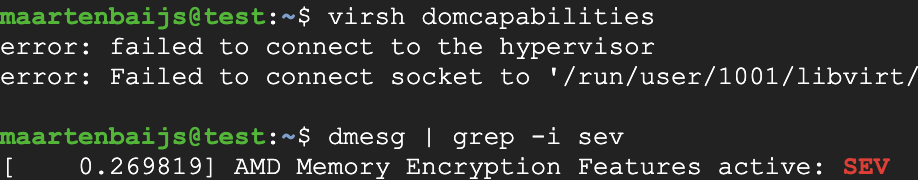
\includegraphics[width=0.6\linewidth]{60-second-notice}
    \caption{60-second notice before a Confidential VM is stopped.}
    \label{fig:60-second-notice}
\end{figure}

\subsection{AMD EPYC} 
Google's Confidential VMs use the AMD EPYC Secure Encrypted Virtualization (SEV) 
to deliver hardware memory encryption (AES-128) to the VM 
while still delivering good performance \citep{amd_amd_2022, amd_secure_2019}. 

“AMD’s Secure Encrypted Virtualization (SEV) is an emerging technology to secure virtual machines (VM) 
even in the presence of malicious hypervisors.” \citep{li_exploiting_2019}.

It locks down the memory with a dedicated per-VM instance key. 
This key is generated and managed by the EPYC processor. 
These keys, in turn, are generated by the AMD Secure Processor during VM creation and reside solely within it.
This means neither Google nor any other VMs running on the host can read your data. 
AMD provides code to validate if you are running inside a SEV environment, 
and provides CPU firmware (updates) on GitHub\footnote{\url{https://github.com/AMDESE }}.

\begin{figure}[!ht]
    \centering
    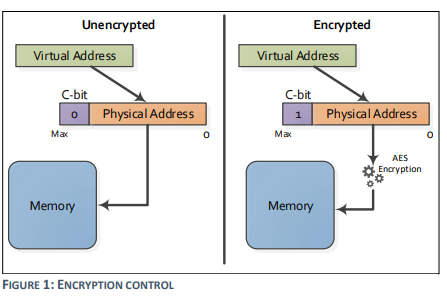
\includegraphics[width=0.6\linewidth]{amd-key-mechanism}
    \caption{AMD SEV Key Mechanism image from \cite{amd_amd_2020}}
    \label{fig:amd-key-mechanism}
\end{figure}



\subsection{AMD SEV}
AMD SEV is part of the Trusted Execution Environment (TEE) design 
and organized in the Confidential Compute Consortium 
\citep{foundation_members_2020}. 
The TEE aims to create a trust stack, 
where the various CPU manufacturers apply a different approach 
\citep{eckert_kick-off_2020,kohlbrenner_building_2020}. 

A list of non-trusted threat vectors are: 
“Cloud operators, processor firmware, SMM (System Management Mode), 
host OS and its hypervisor, all external PCI(e) devices, and more.” 
\citep{chamarthy_challenges_2020}.

\begin{figure}[!ht]
    \centering
    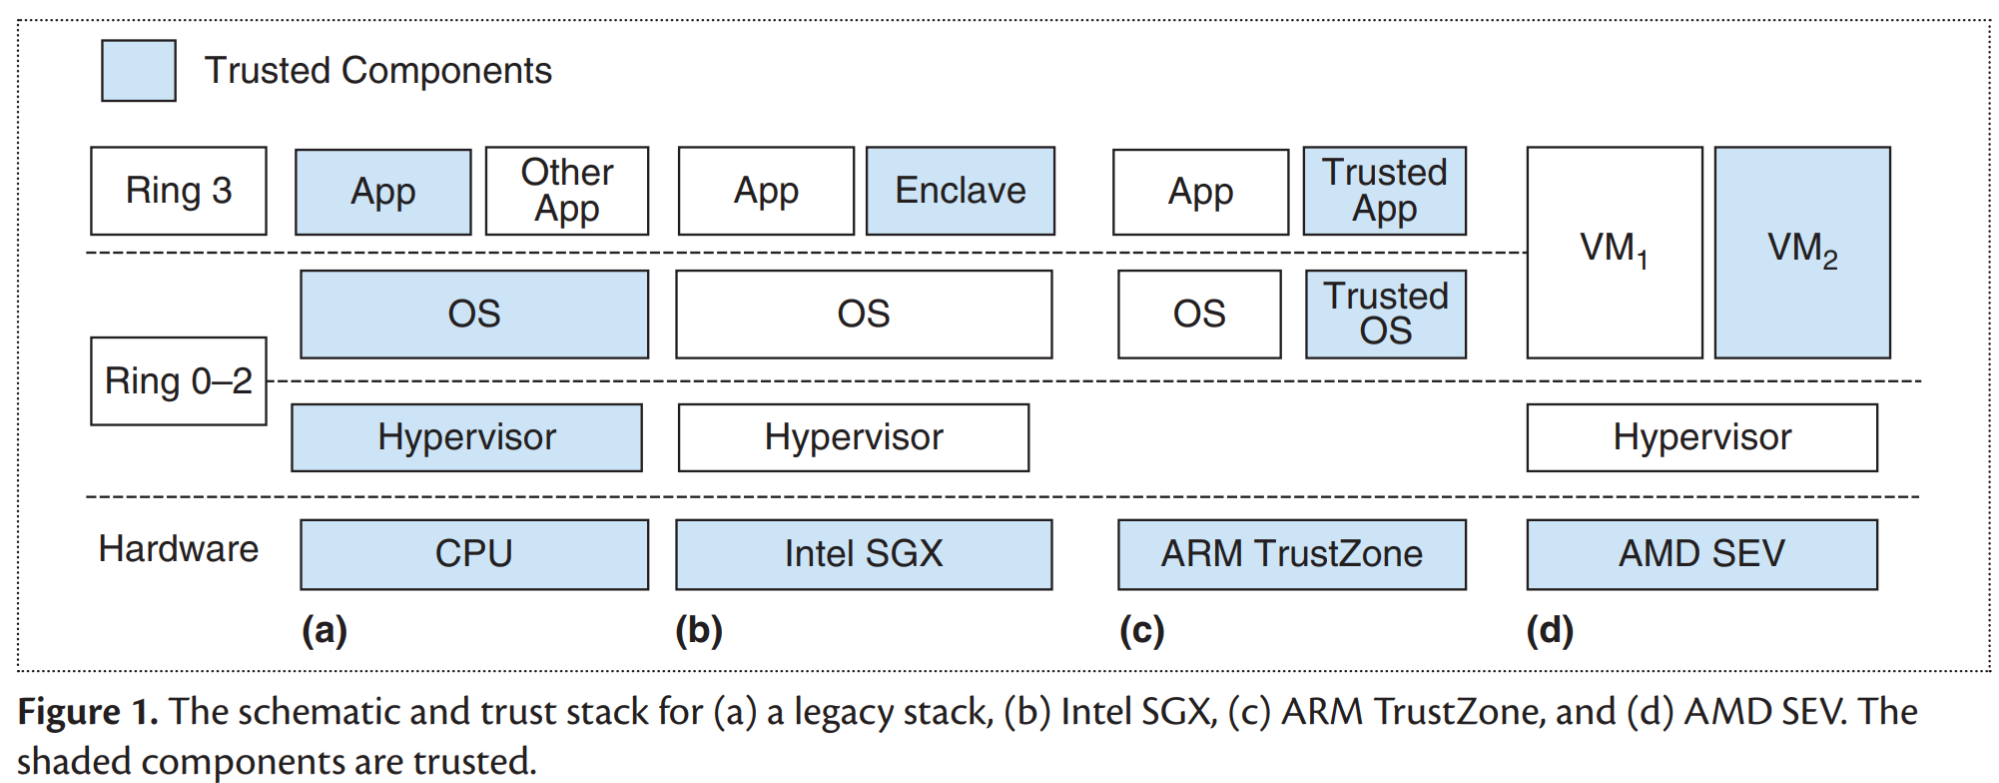
\includegraphics[width=0.7\linewidth]{threat-factors}
    \caption{Threat-factors in the context of Confidential compute 
    image from \cite{kohlbrenner_building_2020}}
    \label{fig:threat-factors}
\end{figure}


\subsection{AMD SEV versions}
Confidential VM at Google Cloud uses the basic version of 
AMD Secure Encrypted Virtualization called “SEV” (EPYC 7001, Napels). 
AMD also offers more advanced versions of this technology called 
SEV-ES (Encrypted State, EPYC 7002, Rome) 
and the newer SEV-SNP (Secure Nested Paging, EPYC 7003, Milan)
\citep{cutress_amd_2021,wikichip_contributors_epyc_2021,kennedy_google_2020}.

\begin{figure}[!ht]
    \centering
    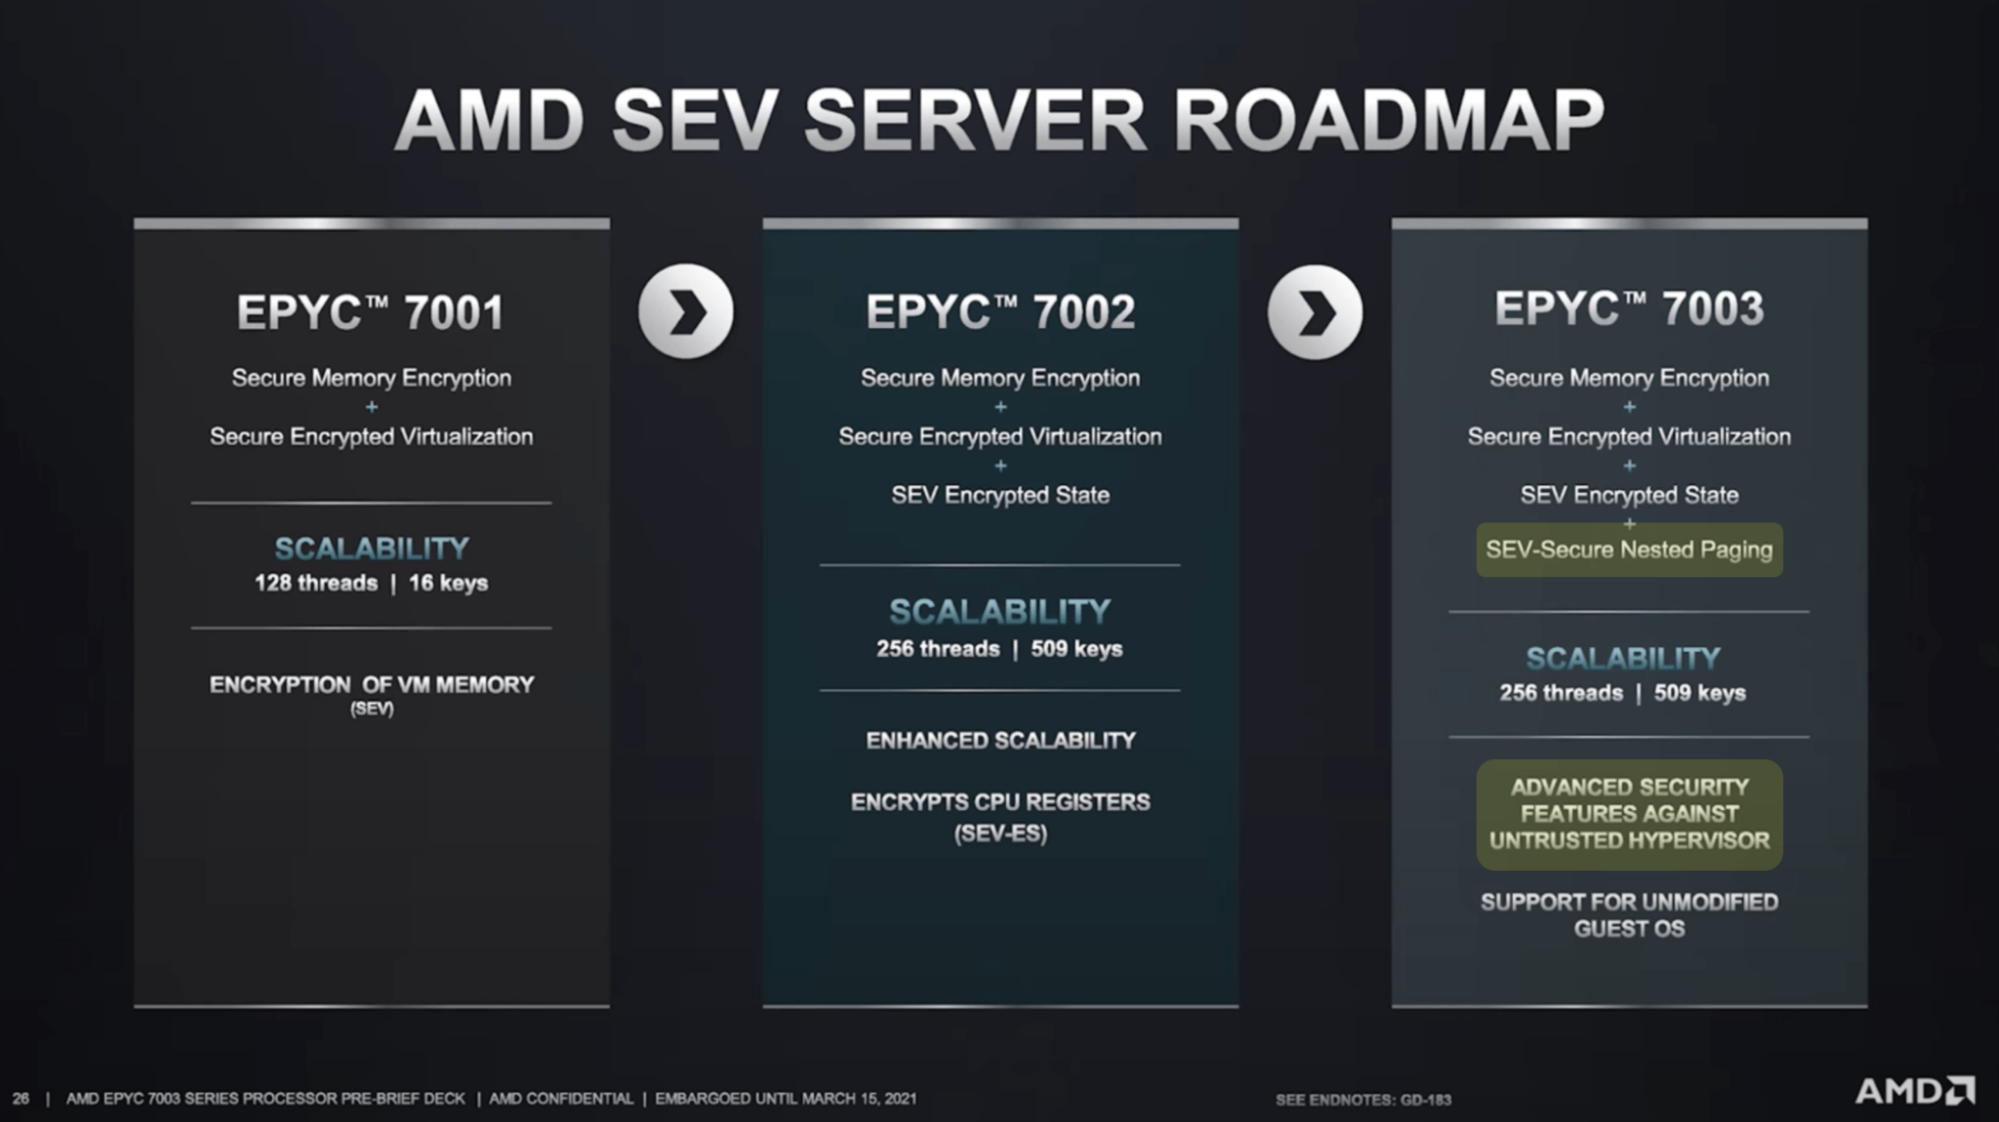
\includegraphics[width=0.9\linewidth]{amd-sev-roadmap}
    \caption{AMD SEV Server Roadmap image from \cite{razavidinani_amd_2021}}
    \label{fig:amd-sev-roadmap}
\end{figure}


“A key thing to understand here is that AMD's SEV technology 
protects data from theft by other code or users on the host box. 
[but]
There is no integrity protection, 
so a compromised hypervisor or rogue Googler could scribble over 
an SEV-protected VM's memory and disrupt, end, or meddle 
with the operation of the Confidential Virtual Machine. 
To prevent malicious reading and writing, 
you need AMD's just-unveiled SEV-SNP technology …” 
\citep{nichols_match_2020,mms_securing_2015}.

Google has started to utilize the EPYC 7003 Milan chips 
for their C2D instances \citep{czop_introducing_2022}. 
However, the ES and SNP versions 
are not supported yet on Confidential Compute at GCP. 


\subsection{AMD SEV versions - threat mitigation overview}
The table below is provided by AMD 
and gives an overview of the various attacks 
that can be mitigated using this technology differentiated per AMD SEV version. 
Next to the whitepaper of AMD on SNP \citep{amd_amd_2020}
there is also a nice presentation by AMD Security Architect 
David Kaplan \citep{kaplan_upcoming_2019} on the extra features of SNP. 

\begin{figure}[!ht]
    \centering
    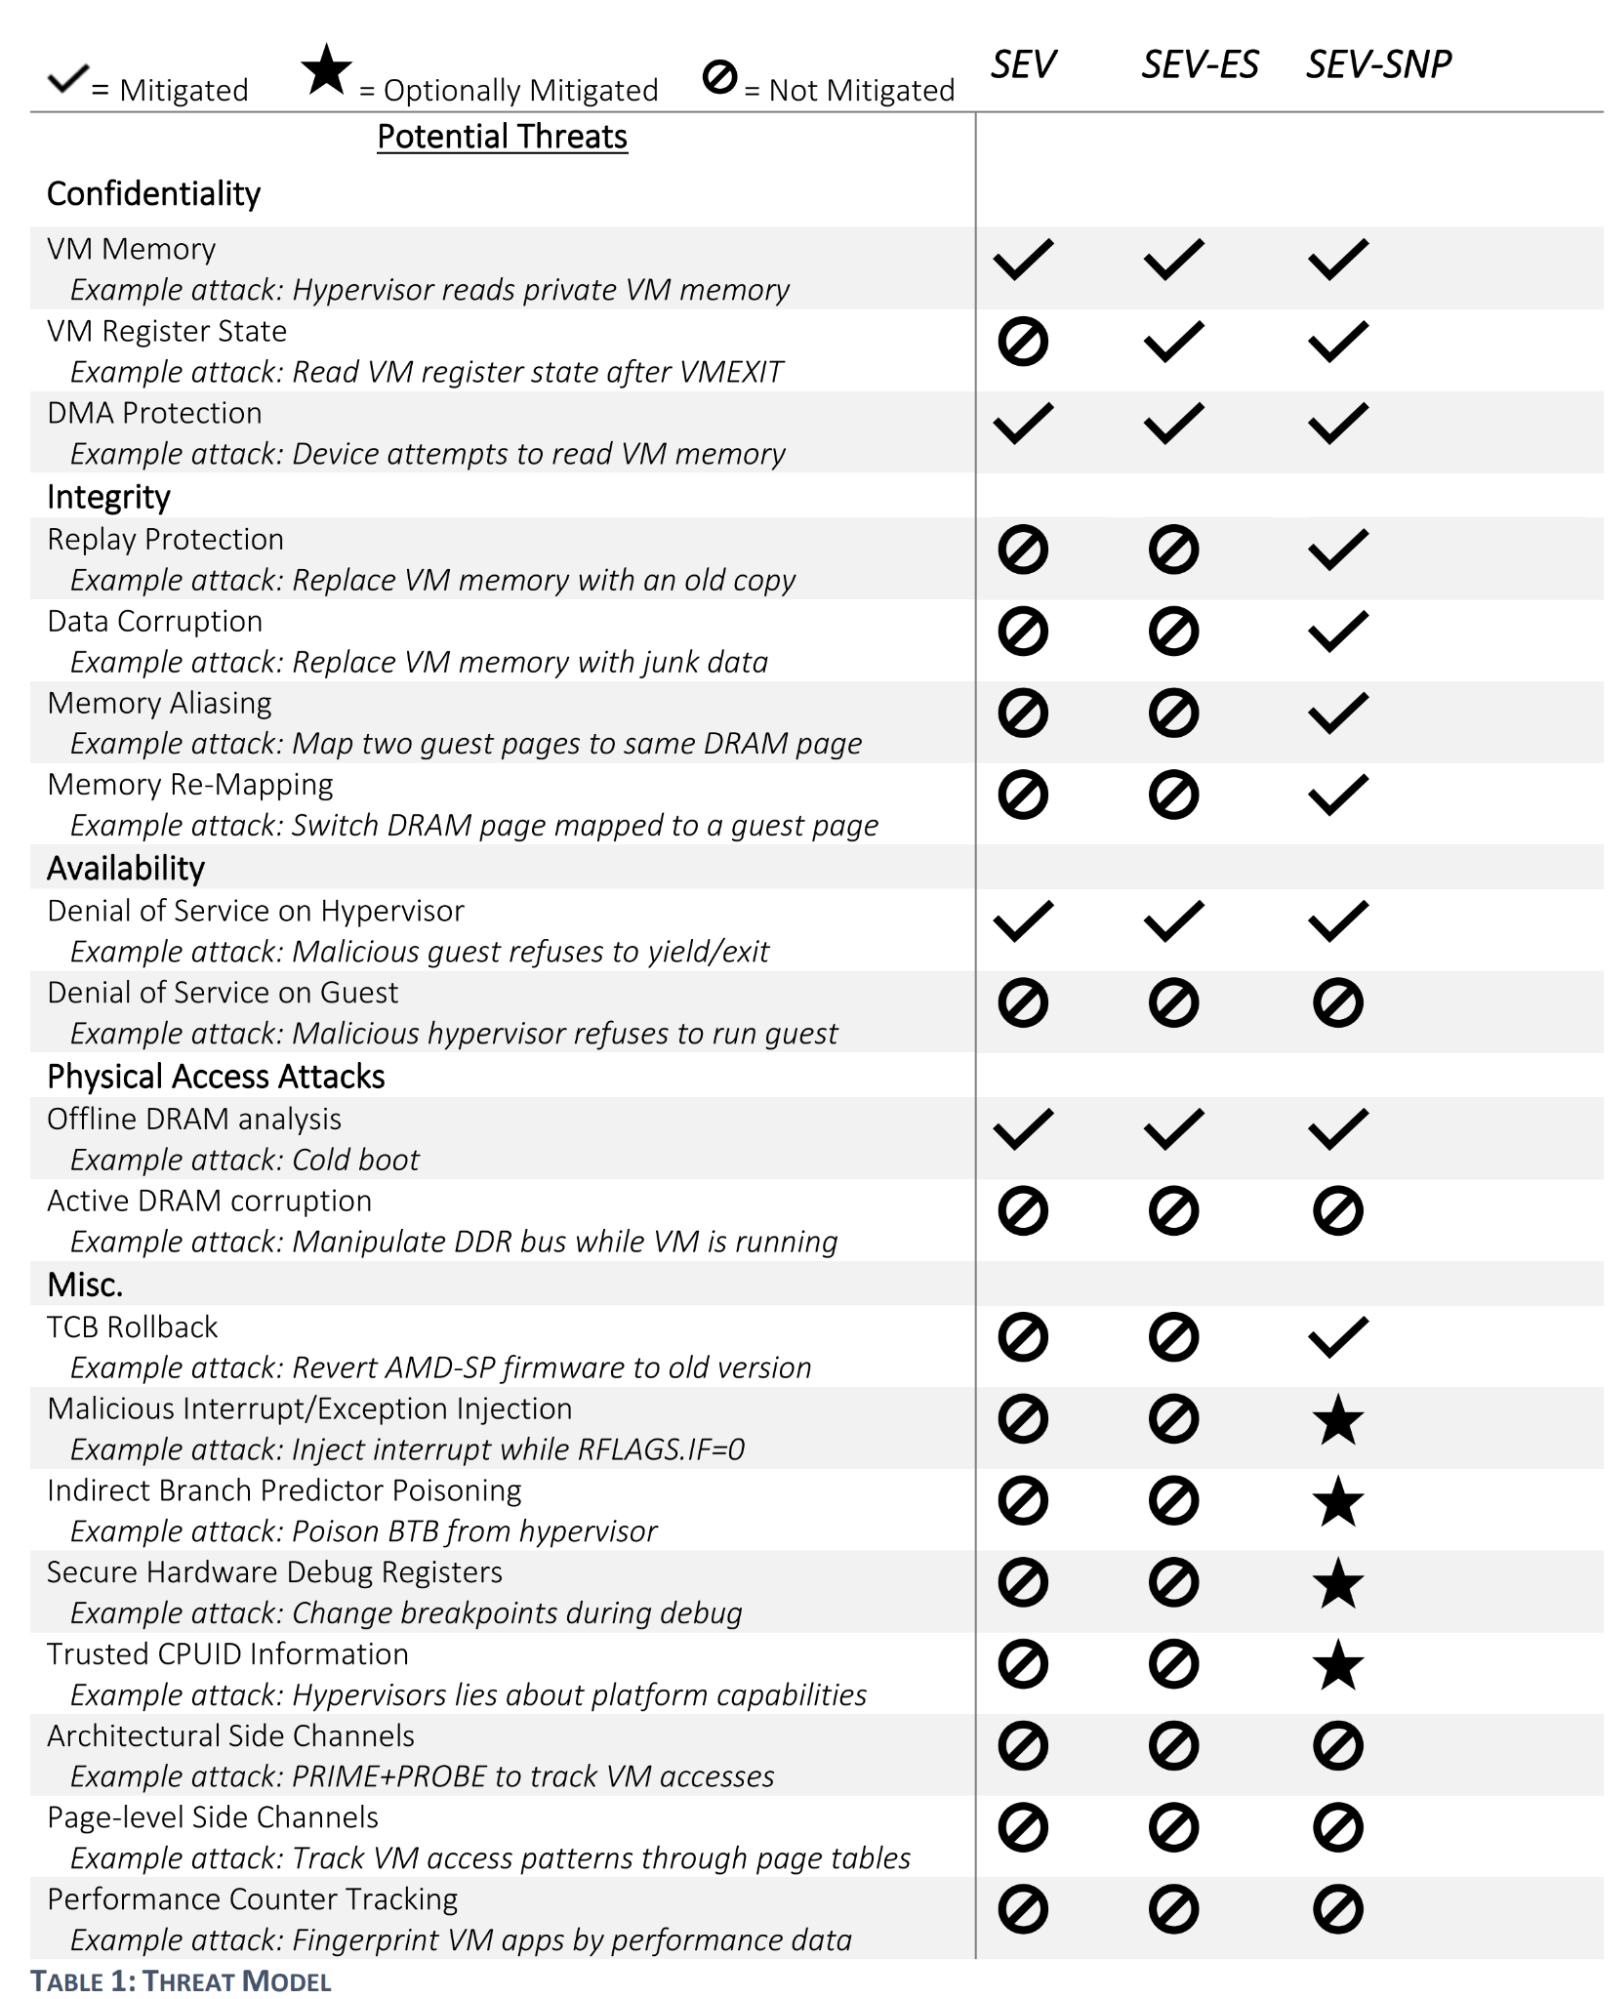
\includegraphics[width=0.9\linewidth]{threat-mitigation-overview}
    \caption{Threat mitigation overview image 
     from \cite{larabel_amd_2022} and is table 1 from \cite{amd_amd_2020}}
    \label{fig:threat-mitigation-overview}
\end{figure}

 

\subsection{GCP - Log Events}

\subsubsection{sevLaunchAttestationReportEvent}
Launch attestation reports are used to validate 
that a Confidential VM is launched. 
That means that the hypervisor created a VM 
with the AMD SEV policies enabled. 
This report event is verified by Google’s hypervisor 
and exposed to the user as a log message.

A launch attestation report event contains information such as the following

\textbf{integrityEvaluationPassed: }\\
The result of an integrity check performed by the Virtual Machine Monitor 
on the measurement computed by AMD SEV.

\textbf{sevPolicy: }\\
The AMD SEV policy bits set for this VM; 
policy bits are set at Confidential VM launch to enforce constraints such as whether debug mode is enabled.

The following screenshot shows a typical launch attestation report:

\begin{figure}[!ht]
    \centering
    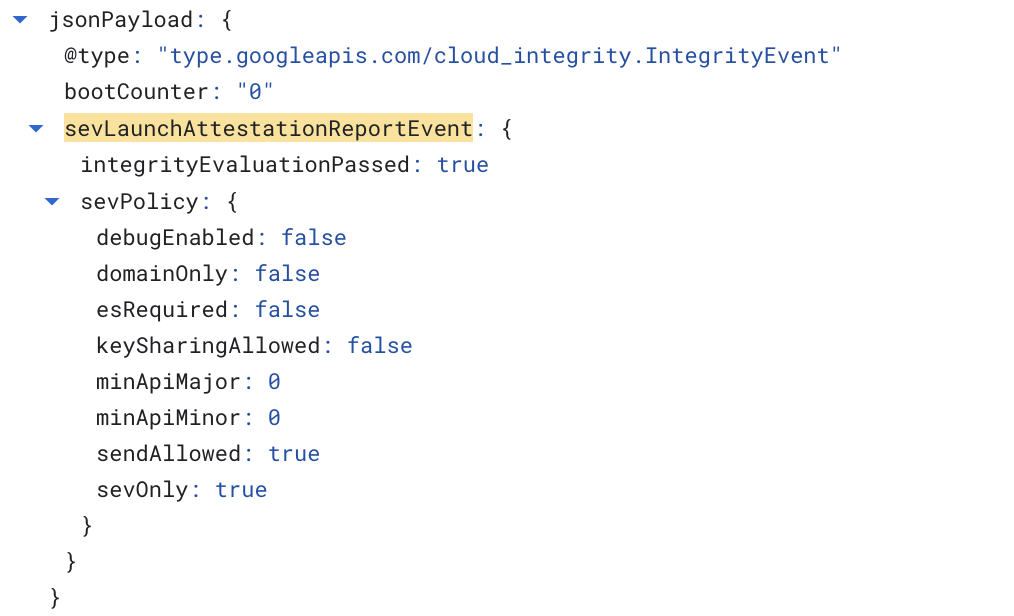
\includegraphics[width=0.7\linewidth]{launch-attestation-report}
    \caption{screenshot attestation report}
    \label{fig:launch-attestation-report}
\end{figure}


\subsection{Verifying AMD SEV is enabled from inside the VM }
Confidential VM uses AMD Secure Encrypted Virtualization (SEV). 
To verify that Confidential Computing is enabled, 
we can use the dmesg logs on your VM 
\citep{marsden_using_2019}. 

\begin{figure}[!ht]
    \centering
    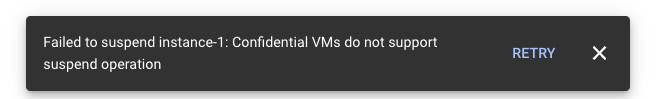
\includegraphics[width=0.6\linewidth]{dmesg-log-message}
    \caption{daemon message attestation log entry}
    \label{fig:dmesg-log-message}
\end{figure}

Next to validating VM kernel messages you can use the 
SEV-Tool\footnote{\url{https://github.com/AMDESE/sev-tool  }} 
to retrieve CPU information as part of the 
AMD toolkit\footnote{\url{https://github.com/AMDESE/sev-guest/blob/main/docs/guest-owner-setup.md }}.

Finally, 
SEV-SNP introduces an API to request the attestation report 
of the secure processor without involvement from the Hypervisor. 
Your VM can use the sev-guest\footnote{\url{https://github.com/AMDESE/sev-guest }} 
tool to request to do so. 
However, the SEV-SNP API is not yet available on GCP (source needed).

\subsubsection{AMD SEV demo encrypted state validation}
There is demo code created by SalrasShid123\footnote{\url{https://github.com/salrashid123/gcp_cc_sev_demo }} on how to use the AMD tooling. 